\input{javapractstyle}
\author{Pieter~van~den~Hombergh}
\title{SEN1 practical task\\State machine using enums\\
  testing using mocks}
\begin{document}
\begin{multicols}{2}
  \maketitle
  \section*{Gum balls as Olifantys}
  \begin{center}
    \begin{Figure}
    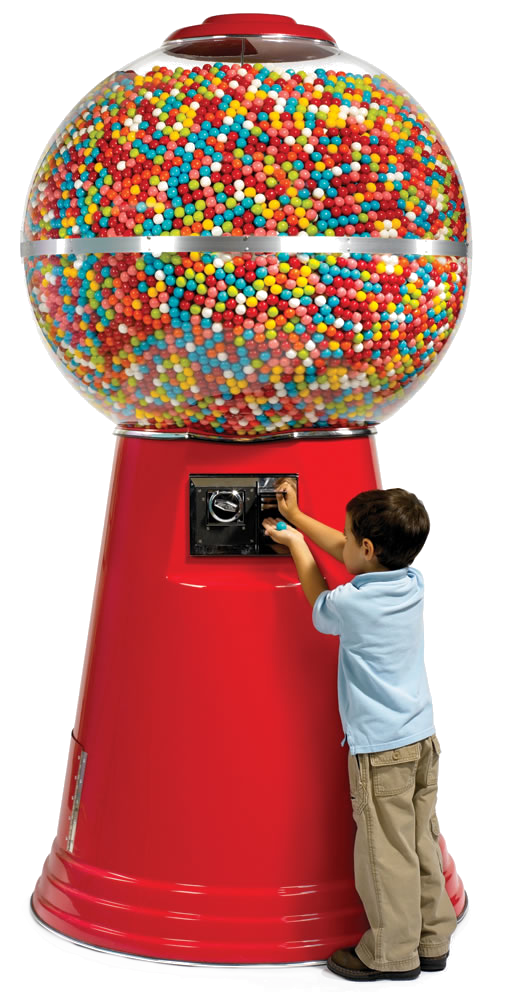
\includegraphics[width=.9\linewidth]{figures/gumballmachine}
    \captionof{figure}{Think Bigger?? Some would like their balls bigger.}
  \end{Figure}
\end{center}

  \subsection*{Learning goals}
  This task has the following learning goals:
  \begin{itemize}
  \item Using enum as state pattern implementation. (enum)
  \item Use Mocking of input and out streams with
    ByteArrayOutputStream. (io streams)
  \item Use of mockito to monitor calls on collaborator.
  \item Optional: use of maven to resolve dependencies.
  \end{itemize}

  The idea of the state machine comes from the book Head First Patterns.


  \subsection*{Design}
  Olifantys has gum ball machines, selling olifantys balls, the mother
  of all gumballs.

  You will write tests and implement a state machine using enums.
  The state machine should support the following behavior:

  The state machine starts in the filled state, filled with a number of
  balls determined by a constructor parameter.

  \subsection*{Behavoir}
  The state model (state diagram) can be found in
  figure~\ref{behavior}.
  We have four states:
  \begin{description}
  \item[SoldOut] No balls.
  \item[NoCoin] No coin in coin slot.
  \item[HasCoin] A coin in coin slot.
  \item[Winner] The customer is lucky and should get an extra ball.
  \end{description}
  (excluding the initial pseudo state) and three events:
  \begin{description}
  \item[refill] New balls in machine, (maybe also remove collected
    coins).
  \item[insertCoin] Put a coin in slot.
  \item[ejectCoin] Get the coin back.
  \item[draw] Pull to get a ball.
  \end{description}

  The implementation should be done with en enum and one enum constant
  (value) for each of the said states.
  The method all have as first parameter the context, which is the
  statemachine context. (The class whose behavior you are implementing).

  The context has a few methods and fields which can be seen in the
  class diagram in figure~\ref{classdiagram}

  \subsection*{Test driven where applicable}
  Instead of a main program that is not very useful, write tests
  for the state enum, using the following concepts:

  In the test packages, implement a mocked PrintStream, which instead of
  writing to an output channel or file, writes (appends) to a string.
  See earlier (Java 2) lesson demo for the idea.
  Then instead of using the State machine in the business package,
  create a mock using Mockito. 

\subsection*{Hints and Tips}
The state-enum implements the \Code{State} interface as seen in
figure~\ref{classdiagram}.
\lstinputlisting[title={State interface}]{code/State.java}
You can have multiple approaches here:
\begin{itemize}
\item Leave all methods abstract en only implement them in the values.
\item Implement all methods as normal methods and overwrite only those
  that are different per instance.
\item A compromise between the two above, saving double work, or
  possible \textit{copy and waste} programming.
\end{itemize}
In this concrete case you do best with the second approach, because
even empty implementations as normal methods are useful because
effectively, the method will have no effect which is quite the same as
ignoring the event. It can also be useful to let the default methods
throw exceptions if for instance you want to make certain method calls
in some states illegal. This is not what we use, but might be
applicable in other situations.

\lstinputlisting[title={State implemented as enum, fragments}]{code/StateEnum.java}

\end{multicols}

\begin{figure}[htbp]\centering
  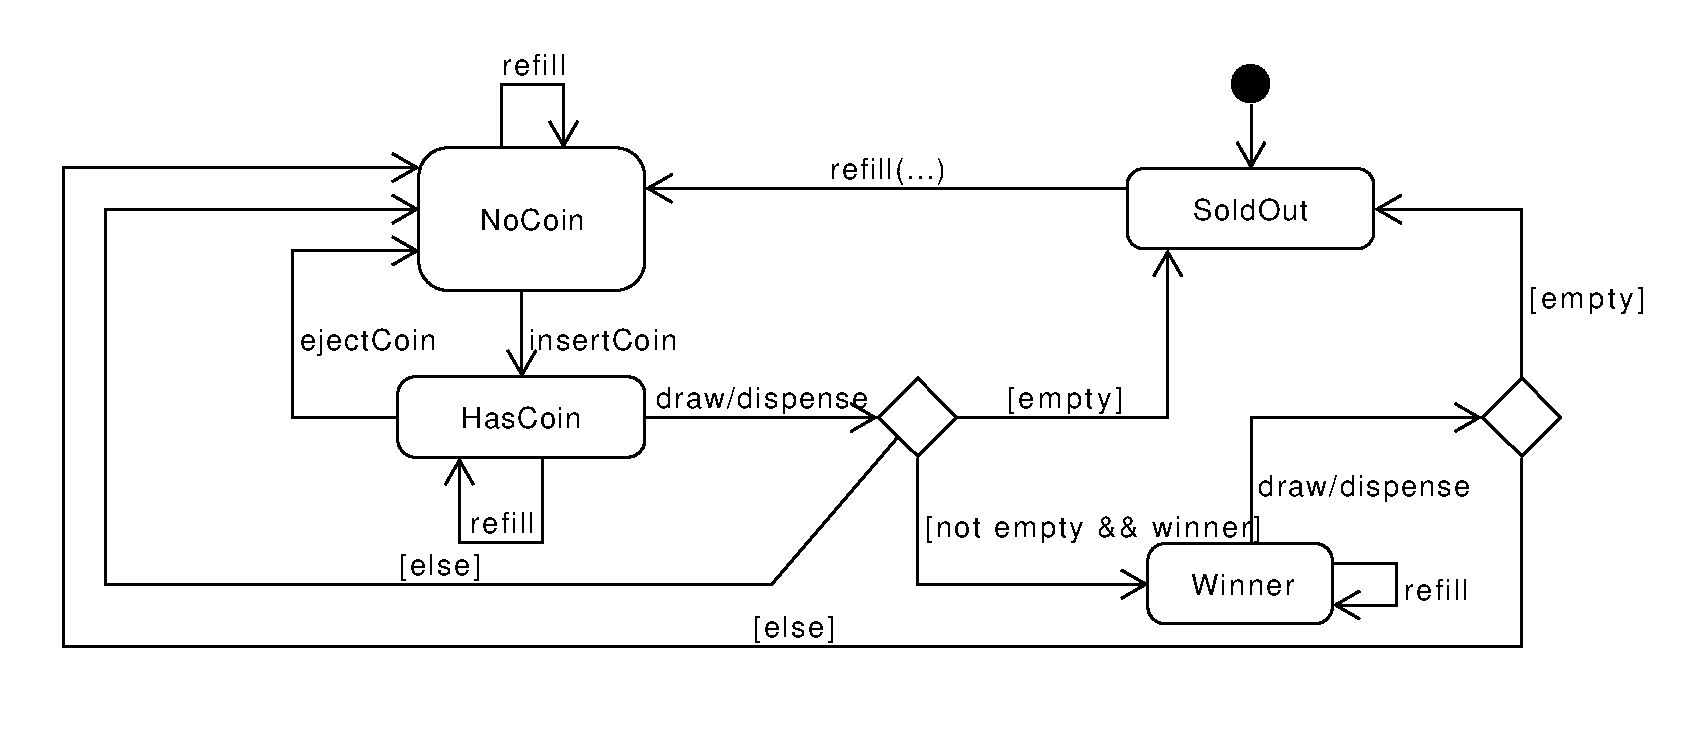
\includegraphics[width=.9\linewidth]{figures/statemachine}
  \caption{\label{behavior}behavior}
\end{figure}

\begin{figure}[htbp]\centering
  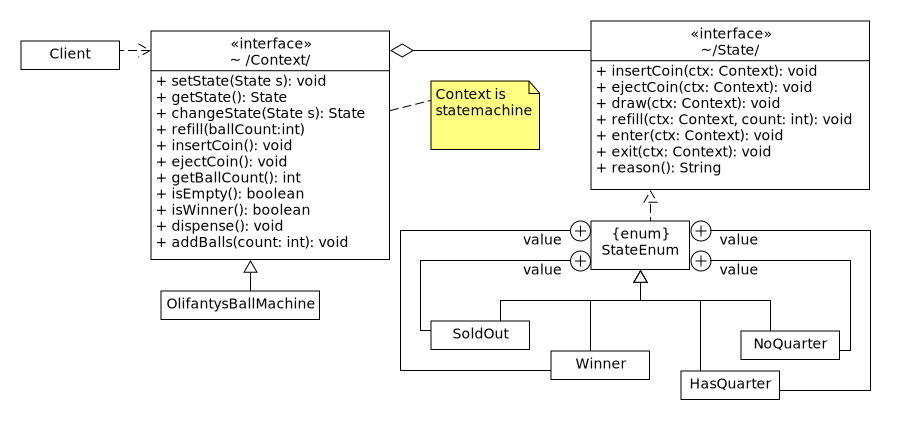
\includegraphics[width=.9\linewidth]{figures/context}
  \caption{\label{classdiagram}State classes and context}
\end{figure}

\label{LastPage}
\end{document}
